\chapter{Acoplamiento Evanescente No Simétrico}
\label{cap:asymmetric}

Los modelos discretos en fotónica, como la teoría de modos acoplados (CMT), suelen asumir acoplamientos simétricos entre guías de onda, es decir, que la constante de acoplamiento entre dos sitios \( C_{i \to j} \) es igual a \( C_{j \to i} \). Esta suposición garantiza la hermiticidad del Hamiltoniano efectivo y suele estar justificada cuando las guías son idénticas y lo suficientemente separadas. Sin embargo, esta simetría puede romperse de forma inherente en sistemas reales, incluso en ausencia de pérdida o ganancia, cuando las guías presentan diferentes perfiles de índice de refracción \cite{nonsymm}.

\section{Origen de la dinámica no simétrica}

El acoplamiento evanescente entre guías de onda se produce por la superposición de las colas modales fuera del núcleo de confinamiento. Cuando dos guías tienen distintos contrastes de índice (\( \Delta n_1 \ne \Delta n_2 \)), los modos guiados presentan colas evanescentes con diferente amplitud y extensión, lo que induce un acoplamiento direccionalmente desigual: \( C_{1 \to 2} \ne C_{2 \to 1} \).

Este comportamiento \textit{no simétrico} puede cuantificarse mediante la teoría de modos acoplados generalizada y no ortogonal, desarrollada en la sección~\ref{cap:CMTteo}, donde se incluye el efecto de solapamiento modal a través de la matriz \( \hat{P} \).

Considerando un dímero compuesto por dos guías no idénticas, las ecuaciones dinámicas para las amplitudes modales se escriben (véase la ecuación~(\ref{eqn:non-ortho-CMT-eqs})) como:
\begin{equation}
	-i
	\frac{d}{dz}
	\begin{pmatrix}
		P_{11} & P_{12} \\
		P_{12} & P_{22}
	\end{pmatrix}
	\begin{pmatrix}
		u_1 \\
		u_2
	\end{pmatrix}
	=
	\begin{pmatrix}
		H_{11} & H_{12} \\
		H_{12} & H_{22}
	\end{pmatrix}
	\begin{pmatrix}
		u_1 \\
		u_2
	\end{pmatrix}
	\iff
	-i\frac{d}{dz}\textbf{v} = \hat{H}' \textbf{v} \ ,
\end{equation}
donde \( \textbf{v} = \hat{P}^{1/2} \textbf{u} \) representa una base ortogonalizada, y \( \hat{H}' = \hat{P}^{-1/2} \hat{H} \hat{P}^{-1/2} \) es el Hamiltoniano efectivo en dicha base. Como \( \hat{H} \) y \( \hat{P} \) son simétricas, \( \hat{H}' \) también lo es, lo que garantiza autovalores reales. Al proponer soluciones del tipo \( \textbf{v}(z) \sim e^{i\lambda z} \), se obtiene el problema generalizado de autovalores $\det(\hat{H} - \lambda \hat{P}) = 0$ .
Es importante destacar que esta base ortogonalizada \( \textbf{v} \) no es accesible experimentalmente: en un montaje real, sólo es posible observar modos localizados en guías individuales, lo cual corresponde a la base física \( \textbf{u} \). Por lo tanto, el análisis experimental de la dinámica debe realizarse en esta base, donde la evolución está gobernada por la matriz de acoplamiento efectiva:
\begin{equation}
	\hat{C} = \hat{P}^{-1} \hat{H} = \frac{1}{P_{11}P_{22} - P_{12}^2}
	\begin{pmatrix}
		P_{22}H_{11} - P_{12}H_{12} & P_{22}H_{12} - P_{12}H_{22} \\
		P_{11}H_{12} - P_{12}H_{11} & P_{11}H_{22} - P_{12}H_{12}
	\end{pmatrix}.
\end{equation}
Este sistema exhibe una dinámica no recíproca: la eficiencia de transferencia de energía depende del canal de entrada. Esta asimetría puede cuantificarse experimentalmente a través del \textit{desbalance de intensidad}, definido para cada excitación \( i = L, R \) como:
\begin{equation}
	I^i(z) \equiv \frac{P^i_1(z) - P^i_2(z)}{P^i_1(z) + P^i_2(z)} \ ,
\end{equation}
y su promedio absoluto como:
\begin{equation}
	\bar{I}(z) \equiv \frac{|I^L(z) + I^R(z)|}{2} \ .
\end{equation}
La cantidad \( \bar{I}(z) \) resulta especialmente útil para detectar asimetrías globales en la dinámica: cualquier desviación de cero implica una evolución no simétrica, revelando la presencia de acoplamientos evanescentes no recíprocos.

\section{Validación Numérica y Comparación con CMT}

Utilizando el método de Expansión en Modos Normales (EME) y resolución numérica de Helmholtz en 2D, se calcularon los modos propios y los acoplamientos efectivos. Se comprobó que la teoría de CMT corregida predice con precisión la dinámica observada, incluso en regímenes de acoplamiento fuerte y desintonizados significativos. En particular, la razón \( C_{21}/C_{12} \) permite cuantificar el grado de no simetría.
\begin{figure}[H]
	\centering
	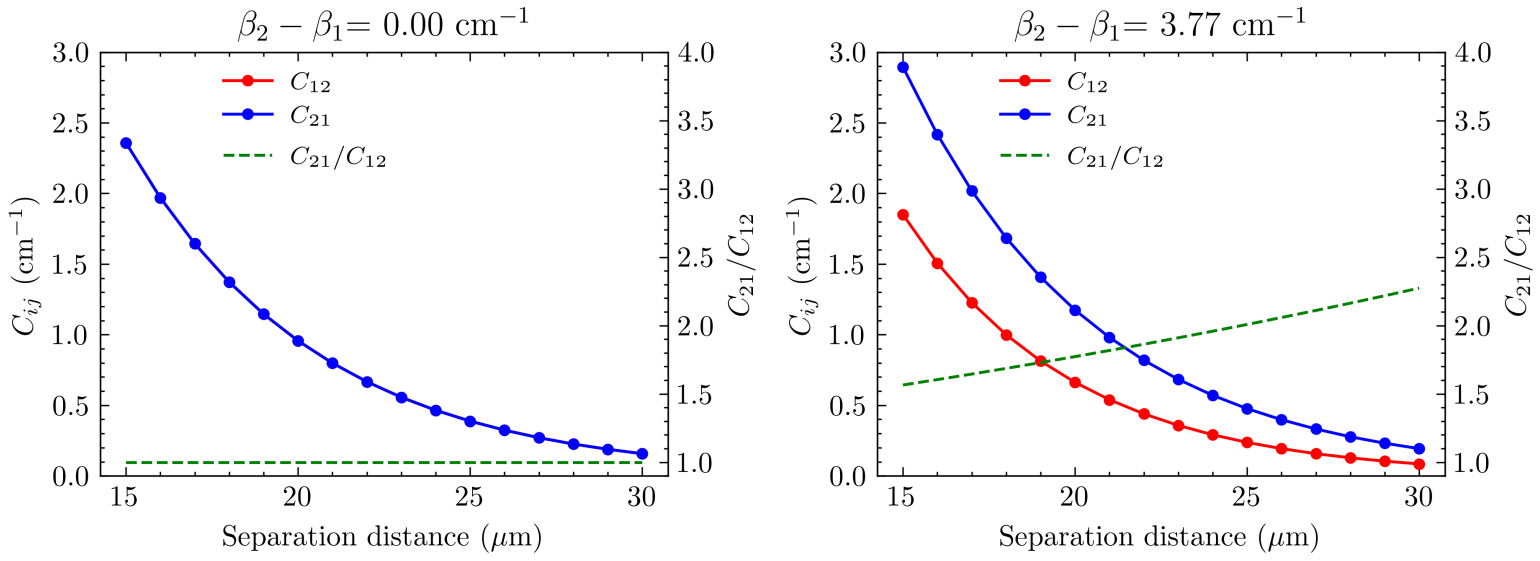
\includegraphics[width=\linewidth]{media/cij-nonortho.png}
	\caption{Constantes de acoplamiento y su razón para un dímero homogéneo (inhomogéneo) en función de la distancia de separación. \label{fig:nonotrho-num}}
\end{figure}
\section{Comprobación Experimental}

Para validar este efecto, se fabricaron dímeros mediante la técnica de escritura por láser femtosegundo descrito en la sección \ref{cap:fs}, variando el canal de entrada \( i \), la potencia de escritura \( P_{g}^i \), la distancia entre guías \( d \), y la longitud de propagación efectiva \( z \). En particular, se exploró el caso \( \Delta P = P_g^1 - P_g^2 = 5\,\mathrm{mW} \), con separación \( d = 18\,\mu\mathrm{m} \). La Figura~\ref{fig:nosymexp} muestra que la excitación de la guía superior favorece la transferencia energética hacia la guía inferior, mientras que la excitación inversa alcanza una distribución energética 1:1 para $z=11$ mm.

\begin{figure}[H]
	\centering
	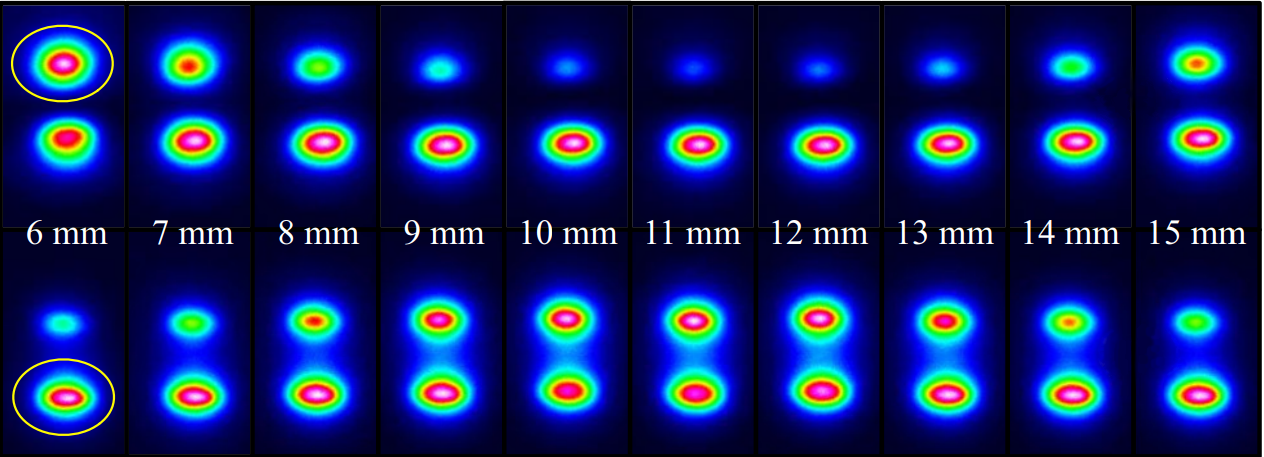
\includegraphics[width=\linewidth]{media/nonsymm-exp.png}
	\caption{Perfiles de salida para distintas longitudes de propagación \( z_i \), excitando la guía superior (izquierda) e inferior (derecha), con \( d = 18\,\mu\mathrm{m} \). \label{fig:nosymexp}}
\end{figure}

Mediante modelos de guías tipo losa (\textit{slab}) y modos TE, se obtienen expresiones analíticas para los acoplamientos:
\begin{equation}
	\frac{C_{21}}{C_{12}} \approx \left( \frac{\Delta n_2}{\Delta n_1} \right)^2 e^{(\gamma_2 - \gamma_1) d} \ ,
\end{equation}
donde \( \gamma_i \) representa el coeficiente de decaimiento evanescente del modo \( i \). Esta expresión muestra que la asimetría aumenta con la separación entre guías y con el contraste de índice. 

\section{Implicancias y Aplicaciones}

Este estudio demuestra que el acoplamiento no simétrico es un fenómeno físico intrínseco en sistemas fotónicos realistas, aún en ausencia de pérdida o ganancia. Sus implicancias incluyen:

\begin{itemize}
	\item \textbf{Ruptura de reciprocidad}: sin requerir materiales magneto-ópticos ni modulación temporal.
	\item \textbf{Asimetría modal}: la desigualdad entre \( C_{ij} \) y \( C_{ji} \) afecta la formación de estados simétricos/antisimétricos y la interferencia.
	\item \textbf{Dispositivos ópticos direccionales}: tales como divisores de haz asimétricos o aislantes ópticos.
	\item \textbf{Extensión a redes}: posibilidad de diseñar redes no Hermíticas con acoplamientos direccionados.
\end{itemize}

En conjunto, estos resultados permiten reinterpretar la teoría de modos acoplados en el contexto de sistemas no ideales, y abren nuevas oportunidades en el diseño de redes ópticas con funcionalidad direccional o topológica.

